\documentclass[10pt]{article}

\usepackage{graphicx}
\usepackage[hmargin=1cm, vmargin=0.6cm]{geometry}
\usepackage{marvosym}
\usepackage{ifsym}

%% Allow use of french caracters
\usepackage[utf8]{inputenc}
\DeclareUnicodeCharacter{2010}{-}

%% Reduce spacing for itemize
\usepackage{enumitem}
	\setitemize{noitemsep,topsep=0pt,parsep=2pt,partopsep=0pt,leftmargin=10pt}

%% Colors for titles, sections, links...
\usepackage[usenames,dvipsnames]{xcolor}
\usepackage{hyperref}
	\definecolor{linkcolor}{HTML}{2000B0} 	% Blue-gray color for links
	\definecolor{gray}{gray}{0.3} 			% Gray for name
	\definecolor{headings}{HTML}{701112} 	% Dark red color for headings
	\hypersetup{colorlinks,breaklinks, urlcolor=linkcolor, linkcolor=linkcolor} % Set up links and colors

%% Format of the section titles
\usepackage{titlesec} % Allows creating custom \section's
\titleformat{\section}{\color{headings}
\scshape\Large\raggedright}{}{0em}{}[\color{black}\titlerule]
\titlespacing{\section}{0pt}{0pt}{5pt} % Spacing around titles

%% No page header or footer
\pagestyle{empty}

%% Length of columns for tables
\newlength{\annee}
\settowidth{\annee}{~~Summer2016~~~~~~~}
\newlength{\texte}
\setlength{\texte}{\textwidth} \addtolength{\texte}{-\annee} \addtolength{\texte}{-2\tabcolsep}

%% Define better + and #
\def\Plus{\texttt{+}}
\newcommand{\Sharp}{{\settoheight{\dimen0}{C}\kern-.05em \resizebox{!}{\dimen0}{\raisebox{\depth}{\#}}}}


\begin{document}

%----------------------------------------------------------------------------------------
%	Titre
%----------------------------------------------------------------------------------------

\begin{minipage}[t]{0.46\textwidth}
{\huge \bf \color{gray} Dr. Martin JACQUET}
~\\[0.4cm]
{\large\bf Doctorat en robotique\\Ingénieur en informatique \par ~~et mathématiques appliquées}
\end{minipage}
\begin{minipage}[t]{0.28\textwidth}
\vspace{0.1cm}
\flushright
\begin{tabular}{c|p{5cm}}
	\raisebox{-4pt}{\textifsymbol{18}}
		& 4D all\'ee Verlaine,\par
		35000 Rennes\\
	\raisebox{0pt}{\Letter}
		& \href{mailto:martin.jacquet@posteo.net}{martin.jacquet@posteo.net} \\
	\raisebox{0pt}{\Letter}
		& \href{mailto:martin.jacquet@inria.fr}{martin.jacquet@inria.fr}
\end{tabular}
\end{minipage}
\begin{minipage}[t]{0.15\textwidth}
\vspace{0.1cm}
\begin{tabular}{c|p{5cm}}
	\raisebox{0pt}{\Mobilefone}
		& \Plus33 (0) 6 47 63 60 50\\
	\raisebox{-0.7pt}{
\includegraphics[scale=0.017]{./images/bday.png}}
		& 28 septembre 1993\\
	\raisebox{-0.5pt}{
\includegraphics[scale=0.033]{./images/car.png}}
		& Permis de conduire\\
\end{tabular}
% \flushright 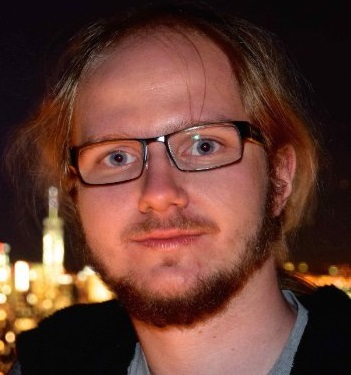
\includegraphics[scale=0.4]{./images/moi.jpg}
\end{minipage}
~\\[0.5cm]

%----------------------------------------------------------------------------------------
%	Expériences
%----------------------------------------------------------------------------------------
~\\[0.2cm]
\section{Expériences \& Formation}

\begin{tabular}{@{}p{\annee}p{\texte}@{}}
	2025-présent \par
	\begin{center}
		
\includegraphics[width=2cm]{./images/inria.jpg}
	\end{center}
	& {\bf Chercheur postdoctoral, à \href{https://www.inria.fr/fr/centre-inria-universite-rennes}{INRIA} - \href{https://team.inria.fr/rainbow/}{équipe RAINBOW}}, Rennes, France \par
	{\small
		% {Avec Dr. Marco Tognon} \par
		\begin{itemize}
			\item Interaction physique basée sur la perception avec des robots aériens
			\item Intégration d'un estimateur d'état lidar-inertiel embarqué
		\end{itemize}
	}
\end{tabular}
\par
\begin{tabular}{@{}p{\annee}p{\texte}@{}}
	2020-présent \par
	& {\bf Enseignant vacataire} \par
	{\small
	\begin{itemize}
		\item À \href{http://www.enseeiht.fr/en/index.html}{INP-ENSEEIHT} : 
			\begin{itemize}
				\item[-] (2020) 21 heures de travaux pratiques - Programmation Android
				\item[-] (2021) 31 heures de travaux dirigés et pratiques - Programmation C, Programmation Android
			\end{itemize} 
		\item À \href{https://www.ntnu.edu/en/home}{NTNU} : (2023) 10 heures de cours et TP - Développement ROS
		\item À \href{https://www.ens-rennes.fr/}{ENS Rennes} : 
			\begin{itemize}
				\item[-] (2025) 6 heures de cours - Robotique aérienne : modélisation et contrôle
				\item[-] (2026) 28 heures de cours et TP - Commande non linéaire
			\end{itemize} 
	\end{itemize}
	}
\end{tabular}
\par
\begin{tabular}{@{}p{\annee}p{\texte}@{}}
	2023-2025 \par
	\begin{center}
		
\includegraphics[width=2cm]{./images/ntnu.pdf}
	\end{center}
	& {\bf Chercheur postdoctoral, à \href{https://www.ntnu.edu/en/home}{NTNU} - \href{https://www.autonomousrobotslab.com/}{Autonomous Robots Lab}}, Trondheim, Norvège \par
	{\small
		% {Avec Prof. Kostas Alexis} \par
		\begin{itemize}
			\item Projet européen EU-Digiforest
			\item Méthodes de contrôle basées sur la perception pour la navigation sans collision en environnements inconnus, complexes et encombrés
			\item Apprentissage profond pour representation implicite d'état/environment (SDF, CBF neurales...)
			\item Participation à des campagnes de tests terrain : déploiement matériel, opérateur de mission
		\end{itemize}
	}
\end{tabular}
\par
\begin{tabular}{@{}p{\annee}p{\texte}@{}}
	2019-2022 \par
	\begin{center}
		
\includegraphics[width=1.5cm]{./images/laas.png}
	\end{center}
	& {\bf Doctorat en robotique, au \href{https://www.laas.fr/en/}{LAAS-CNRS} - \href{https://www.laas.fr/en/teams/ris/}{groupe RIS}}, Toulouse, France \par
	{\small
		{\bf Methodes pour contrôle prédictif en ligne de robots aeriens multi-rotors pour des tâches orientées perception et sujet à des contraintes capteurs/moteurs} \par
		% {Directeur : Prof. Antonio Franchi} \par
		\begin{itemize}
			\item Projet ARN-MuRoPhen
			\item Commande prédictive non linéaire, Méthodes de perception active, Systèmes multi-robots aériens
	     	% \item Participation à la compétition robotique \href{https://www.mbzirc.com}{MBZIRC 2020} : développement logiciel lié à la perception
		\end{itemize}
	}
\end{tabular}
\par
\begin{tabular}{@{}p{\annee}p{\texte}@{}}
  	2017-2018 \par
  	\begin{center}
	  
\includegraphics[width=1.5cm]{./images/laas.png}
	\end{center}
  & {\bf Ingénieur de recherche au \href{https://www.laas.fr/en/}{LAAS-CNRS} - \href{https://www.laas.fr/en/teams/rap/}{groupe RAP}}, Toulouse, France \par
    {\small
		\begin{itemize}
			\item Projet collaboratif avec l'Institut Français de la Vigne et du Vin (Gaillac) et Naïo Technologies (Toulouse)
			\item Détection basée sur l'apprentissage profond de troncs et maladies foliaires sur images de vignes
		    % \item Programmation Python et C\Plus\Plus, bibliothèques Keras et TensorFlow
		\end{itemize}
	}
\end{tabular}
\par
\begin{tabular}{@{}p{\annee}p{\texte}@{}}
  Été 2016 \par
  	\begin{center}
  		
\includegraphics[width=1.5cm]{./images/atos.jpg}
	\end{center}
	& {\bf Stage ingénieur de 6 mois chez \href{https://atos.net/en/}{ATOS}}, Toulouse, France \par
    {\small
		\begin{itemize}
			\item Conception et déploiement d'algorithmes de détection et de suivi d'icebergs sur images satellites
		    \item Programmation C\Plus\Plus, technologies web (API, base de données, déploiement Docker...)
		\end{itemize}
	}
\end{tabular}
\par
\begin{tabular}{@{}p{\annee}p{\texte}@{}}
	Été 2015 \par
	\begin{center}
  		
\includegraphics[width=1.5cm]{./images/irit.png}
	\end{center}
	& {\bf Stage de recherche de 3 mois à l'\href{https://www.irit.fr/?lang=en}{IRIT}}, Toulouse, France \par
	{\small
		Recherche de symétries pour la compression de maillages 3D.
		\begin{itemize}
			\item Transposition d'algorithmes 2D vers la 3D pour l'extraction de caractéristiques (SIFT)
		    \item Méthodologie d'évaluation statistique
		\end{itemize}
	}
\end{tabular}

% \par
% \begin{tabular}{@{}p{\annee}p{\texte}@{}}
% 	Août 2014 & {\bf Working training period in a Japanese hostel, as a cleaning person.} \par
% 		\small Kamogawa Hotel Mikazuki, Kominato, Chiba, Japan.
% \end{tabular}
\par
\begin{tabular}{@{}p{\annee}p{\texte}@{}}
	2013-2016 \par
	\begin{center}
		
\includegraphics[width=2cm]{./images/n7.png}
		\\ \vskip1mm
		
\includegraphics[width=2cm]{./images/polymtl.jpg}
	\end{center}
	& {\bf \'Ecole d'ingénieur, à l'\href{http://www.enseeiht.fr/en/index.html}{INP-ENSEEIHT}}, Toulouse, France \par
		\small{
			{\bf Département Informatique et Mathématiques Appliquées}
			\begin{itemize}
				\item Traitement de données audio-visuelles - Vision par ordinateur - 3D - Réalité Virtuelle
				\item Mathematique - Statistiques/Probabilités - Algèbre Linéaire algebra - Optimisation
				\item Informatique - Développement logiciel
				\item Semestre à \href{http://www.polymtl.ca/}{Polytechnique Montreal}, Canada; Cours en technologies multimédia  \par
			    % \item 2 months Project : Building a 3D model of a scene from RGBD data
			\end{itemize}
		}
\end{tabular}
% \par
% \begin{tabular}{@{}p{\annee}p{\texte}@{}}
% 	2011-2013
% 	& {\bf Preparatory school,} \small{PSI* (Physics and engineer sciences).}\par
%     \small{Lycée Champollion, Grenoble, France.}
% \end{tabular}
% \par
% \begin{tabular}{@{}p{\annee}p{\texte}@{}}
% 	2011 & {\bf Scientific Baccalauréat}.\par
% 		    \small{Lycée Pierre Termier, Grenoble, France.}
% \end{tabular}

\vfill
\centering{\footnotesize\it Références et informations complémentaires disponibles sur demande}

\newpage
%----------------------------------------------------------------------------------------
%	Publications
%----------------------------------------------------------------------------------------
~\\[0.2cm]
\section{Publications}

\begin{tabular}{@{}p{\annee}p{\texte}@{}}
	\small
	Thèse de doctorat	& {\bf M. Jacquet}, \href{https://theses.fr/2022ISAT0021}{\it Methodes pour contrôle prédictif en ligne de robots aeriens multi-rotors pour des tâches orientées perception et sujet à des contraintes capteurs/moteurs}
\end{tabular} \par
\begin{tabular}{@{}p{\annee}p{\texte}@{}}
	\small
	ICRA'20				& {\bf M. Jacquet}, G. Corsini, D. Bicego, A. Franchi, \href{https://doi.org/10.1109/ICRA40945.2020.9197281}{\it Perception-constrained and Motor-level Nonlinear MPC for both Underactuated and Tilted-propeller UAVS}
\end{tabular} \par
\begin{tabular}{@{}p{\annee}p{\texte}@{}}
	\small
	RAL	(2021)			& {\bf M. Jacquet}, A. Franchi, \href{https://doi.org/10.1109/LRA.2020.3045654}{\it Motor and Perception Constrained NMPC for Torque-Controlled Generic Aerial Vehicles} \par
						--Finaliste pour ``Best Paper Award in Unmanned Aerial Vehicles'' à ICRA'21
\end{tabular} \par
\begin{tabular}{@{}p{\annee}p{\texte}@{}}
	\small
	AIRPHARO'21			& G. Corsini, {\bf M. Jacquet}, AE. Jimenez-Cano, A. Afifi, D. Sidobre, A. Franchi, \href{https://doi.org/10.1109/AIRPHARO52252.2021.9571053}{\it A General Control Architecture for Visual Servoing and Physical Interaction Tasks for Fully-actuated Aerial Vehicles}
\end{tabular} \par
\begin{tabular}{@{}p{\annee}p{\texte}@{}}
	\small
	RAL (2022)			& {\bf M. Jacquet}, M. Kivits, H. Das, A. Franchi, \href{https://doi.org/10.1109/LRA.2022.3143218}{\it Motor-level N-MPC for Cooperative Active Perception with Multiple Heterogeneous UAVs}
\end{tabular} \par
\begin{tabular}{@{}p{\annee}p{\texte}@{}}
	\small
	IROS'22				& {\bf M. Jacquet}, A. Franchi, \href{https://doi.org/10.1109/IROS47612.2022.9981643}{\it Enforcing Vision-Based Localization using Perception Constrained N-MPC for Multi-Rotor Aerial Vehicles}
\end{tabular} \par
\begin{tabular}{@{}p{\annee}p{\texte}@{}}
	\small
	IROS'22				& G. Corsini, {\bf M. Jacquet}, H. Das, A. Afifi, D. Sidobre, A. Franchi, \href{https://doi.org/10.1109/IROS47612.2022.9981045}{\it Nonlinear Model Predictive Control for Human-Robot Handover with Application to the Aerial Case}
\end{tabular} \par
\begin{tabular}{@{}p{\annee}p{\texte}@{}}
	\small
	ICRA'24				& {\bf M. Jacquet}, K. Alexis, \href{https://doi.org/10.1109/ICRA57147.2024.10610572}{\it N-MPC for Deep Neural Network-Based Collision Avoidance exploiting Depth Images}
\end{tabular} \par
\begin{tabular}{@{}p{\annee}p{\texte}@{}}
	\small
	IROS'24				& M. Harms, M. Kulkarni, N. Khedekar, {\bf M. Jacquet}, K. Alexis, \href{https://doi.org/10.1109/IROS58592.2024.10802694}{\it Neural Control Barrier Functions for Safe Navigation}
\end{tabular} \par
\begin{tabular}{@{}p{\annee}p{\texte}@{}}
	\small
	ICUAS'25			& N. Misyats, M. Harms, M. Nissov, {\bf M. Jacquet}, K. Alexis, \href{https://doi.org/10.1109/ICUAS65942.2025.11007827}{\it Embedded Safe Reactive Navigation for Multirotors Systems using Control Barrier Functions}
\end{tabular} \par
\begin{tabular}{@{}p{\annee}p{\texte}@{}}
	\small
	ICRA'25				& M. Harms, {\bf M. Jacquet}, K. Alexis, \href{https://doi.org/10.1109/ICRA55743.2025.11127368}{\it Safe Quadrotor Navigation using Composite Control Barrier Functions}
\end{tabular} \par
\begin{tabular}{@{}p{\annee}p{\texte}@{}}
	\small
	IJRR (2025)			& {\bf M. Jacquet}, M. Harms, K. Alexis, \href{https://doi.org/10.1177/02783649251401223}{\it Neural NMPC through Signed Distance Field Encoding for Collision Avoidance}
\end{tabular} \par


%----------------------------------------------------------------------------------------
%	Services editoriaux
%----------------------------------------------------------------------------------------
~\\[0.2cm]
\section{Services éditoriaux}

\begin{tabular}{@{}p{\annee}p{\texte}@{}}
	\bf Relecteur		& 	Revues (T-RO, IJRR, Nature Communications, RAL) \\
	~					& 	Conférences (RSS, ICRA, IROS, ICUAS, ECC)
\end{tabular}


%----------------------------------------------------------------------------------------
%	Compétences techniques
%----------------------------------------------------------------------------------------
~\\[0.2cm]
\section{Compétences techniques}

\begin{tabular}{@{}p{\annee}p{\texte}@{}}
	\bf Scientifiques		& 	Réseaux de neurones, représentations neuronales implicites \par
							Commande optimale non linéaire \par
							Estimation de pose, incertitudes, filtrage de Kalman \par
							Apprentissage profond pour le traitement d'images et de vidéos \par
							Modélisation mathématique, estimation de paramètres physiques \\
	\bf Langages 		& 	Python, {C\Plus\Plus}, C, Matlab \\
	% \bf Software 		& 	ROS, ROS2, GenoM, LateX, Git \\
	% \bf Librairies		& 	PyTorch, OpenCV, Eigen, PCL \\
	\bf Matériel 		& 	Caméras (calibration, acquisition de données), Lidars, IMUs, manipulation de drones sur mesure, électronique de drones
\end{tabular}


%----------------------------------------------------------------------------------------
%	Langues
%----------------------------------------------------------------------------------------
~\\[0.2cm]
\section{Langues}

\begin{tabular}{@{}p{\annee}p{\texte}@{}}
	\bf Français		& Langue maternelle \\
	\bf Anglais 	& C1, communication écrite et orale courante ; {\sc Toeic} obtenu en 2015 (940) \par
		Communication professionnelle quotidienne (équipe internationale) \\
	\bf Espagnol 	& Niveau scolaire (B1) \\
	\bf Japonais 	& Débutant avancé \\
	\bf Norvégien 	& Débutant \\
\end{tabular}


%----------------------------------------------------------------------------------------
%	Informations diverses
%----------------------------------------------------------------------------------------
~\\[0.2cm]
\section{Informations diverses}

\begin{tabular}{@{}p{\annee}p{\texte}@{}}
	% \bf Personal projects &
	% 	Video games prototyping \par
	% 	Hobby software development\\
	\bf Loisirs &
    	Programmation, cyclisme, brassage, jeux de rôle sur table, cinéma, photographie, science-fiction
\end{tabular}
%----------------------------------------------------------------------------------------

\vfill
\centering{\footnotesize\it Références et informations complémentaires disponibles sur demande}

\end{document}
